\chapter{Overview of Main VSM Topologies}\label{chap:vsm-overview}

With the increasing penetration of Inverter-Based Resources (IBRs) and the
diminished involvement of Synchronous Generators (SGs) in energy generation,
existing power systems are experiencing loss of inertia. This loss
significantly impacts two key aspects. Firstly, the absence of kinetic energy in
the system leads to a higher frequency nadir and a faster rate of change in
frequency (RoCoF), thereby affecting power quality and potentially causing the
tripping of generators \cite{alipoor2015power}.

One of the most promising solutions to address these challenges is the
implementation of Virtual Synchronous Machines (VSMs). A VSM is a control
technique applied to the switching patterns of voltage source converters (VSCs),
aiming to replicate the dynamic behavior of SGs.

Among the most notable word on VSMs are from: the VSYNC project
\cite{visscher2008vsg} under the 6th European Research Framework program, the
Virtual Synchronous Machine (VISMA) project \cite{beck2007vsm} at the Institute
of Electrical Power Engineering (IEPE) of Clausthal University of Technology in
Germany, the VSM research team at Kawasaki Heavy Industries (KHIs)
\cite{hirase2013grid}, and the Laboratory for Power Electronics and Electrical
Drives (formerly ISE Lab) at Osaka University \cite{alipoor2015power,
sakimoto2011stabilization, liu2017vsg}. In this chapter, we first provide the
classification  of control methods for power converters, then we provide an
overview and comparison of the topologies developed by aforementioned research
groups and other relevant researchers.

\section{Control Methods of Power Converters}\label{sec:control_methods}

Power converters play a crucial role in integrating renewable energy sources
into the power grid and are primarily classified into two types: grid-forming
and grid-following control \cite{blaabjerg2018control}. Grid-forming converters
maintain a constant voltage and frequency, functioning as ideal voltage sources
capable of standalone operation or synchronizing with other generators. However,
their inability to operate in parallel with other voltage sources limits their
application.

Conversely, grid-following converters, designed to regulate output power by
adjusting the injected current, act as current sources and require an external
voltage reference for stable operation. They are unsuitable for standalone use
due to their reliance on an existing voltage source for support.

Grid-supporting control, a versatile category, extends converter capabilities
for both standalone and grid-integrated operations. It splits into two subtypes:
current-source and voltage-source grid-supporting controls.

Current-source-based grid-supporting control, an evolution of grid-following
control, incorporates droop control for power sharing but still necessitates
connection to a voltage source for system support, similar to grid-following
converters.

Voltage-source-based grid-supporting control, on the other hand, stems from
grid-forming technology. These converters can function independently and in
parallel with other voltage sources, including the main grid, thanks to the
integration of droop control laws. This feature not only facilitates automatic
power sharing but also enables parallel connectivity, making
voltage-source-based grid-supporting converters a highly adaptable and promising
solution for power converter applications.

\begin{figure}[h!]
    \centering
    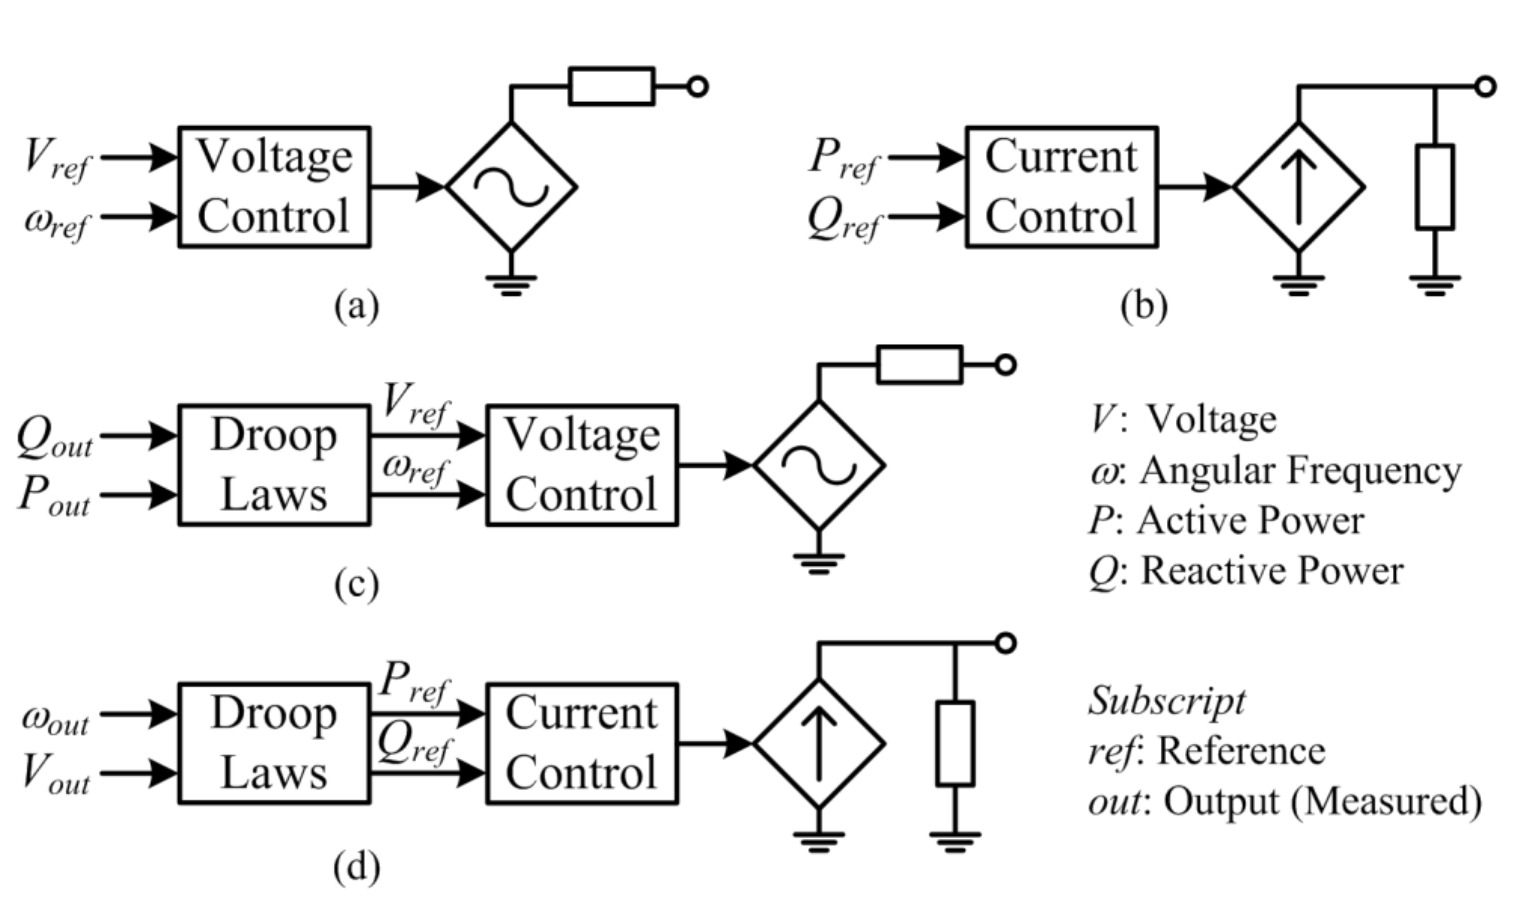
\includegraphics[width=12cm]{images/control_methods.png}
    \caption{Control methods for power converters. (a) Grid-forming control, (b)
    Grid-following control, (c) Voltage-source-based grid-supporting control and
    (d) Current-source-based grid-supporting control \cite{paquette2015virtual}.}
    \label{fig:control_methods}
\end{figure}


\section{VSYNC Project's VSM Topology}\label{sec:VSYNC}

The VSYNC project, initiated under the 6th European Research Framework program,
represents a pioneering effort in implementing virtual inertia control for
inverters. This project's system comprised an energy storage unit, a DC link,
and a power inverter with an output LCL filter connected to an AC electrical
grid \cite{visscher2008vsg}.

The control scheme incorporates a Phase-Locked Loop (PLL) and a current
reference generation circuit. The PLL is used for synchronization with the grid
frequency and for providing an angle reference for the dq transformation.
Meanwhile, the current reference generation circuit generates the reference
current for controlling the inverter's switching pattern through PWM modulation.
The overall control scheme of the VSYNC topology is illustrated in the following
image.

\begin{figure}
    \centering
    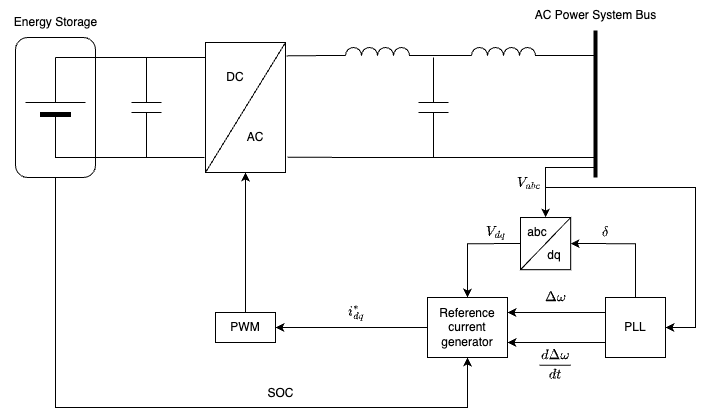
\includegraphics[width=12cm]{images/VSYNC.png}
    \caption{Overall control scheme of the VSYNC topology.}
    \label{fig:VSYNC}
\end{figure}

The current reference is calculated based on the reference active $P^*$ and
reactive $Q^*$ powers, which are calculated according to the SG swing equation
so that the overall system can emulate the SGs inertial response.
\begin{equation*}
    \begin{aligned}
        P^* &= K_{SOC}\Delta SOC + K_P \Delta\omega + K_t \frac{\Delta \omega}{dt}\\
        Q^* &= K_V \Delta V\\
        i_{d}^* &= \frac{V_d P^* - V_q Q^*}{(V_d + V_q)^2}\\
        i_{q}^* &= \frac{V_d Q^* - V_q P^*}{(V_d + V_q)^2}
    \end{aligned}
\end{equation*}

Overall, the VSYNC control scheme is a current-source based grid-supporting control
mechanism, employing a current control loop at the output terminal and using a
PLL to detect grid frequency and provide an angle reference for the dq
transformation. It is important to note that the use of a PLL can negatively
impact control performance under weak AC systems. Furthermore, the VSYNC control
scheme incorporates only the SG swing equation.

\section{IEPE's VSM Topology}\label{sec:VISMA}

The IEPE group has proposed a VSM topology named Virtual Synchronous Machine
(VISMA), which initially utilized a current-source-based approach on a
hysteresis controlled inverter~\cite{beck2007vsm,chen2011improving}.
Subsequently, a voltage-source-based method was suggested to broaden its
applicability to PWM controlled inverters, more prevalent in the
market~\cite{chen2012comparison}. These are referred to as VISMA-Method 1 and
VISMA-Method 2, respectively, with their control schemes depicted in subsequent
figures.


\newpage
\begin{figure}[ht!]
    \centering
    \begin{subfigure}[b]{\textwidth}
        \centering
        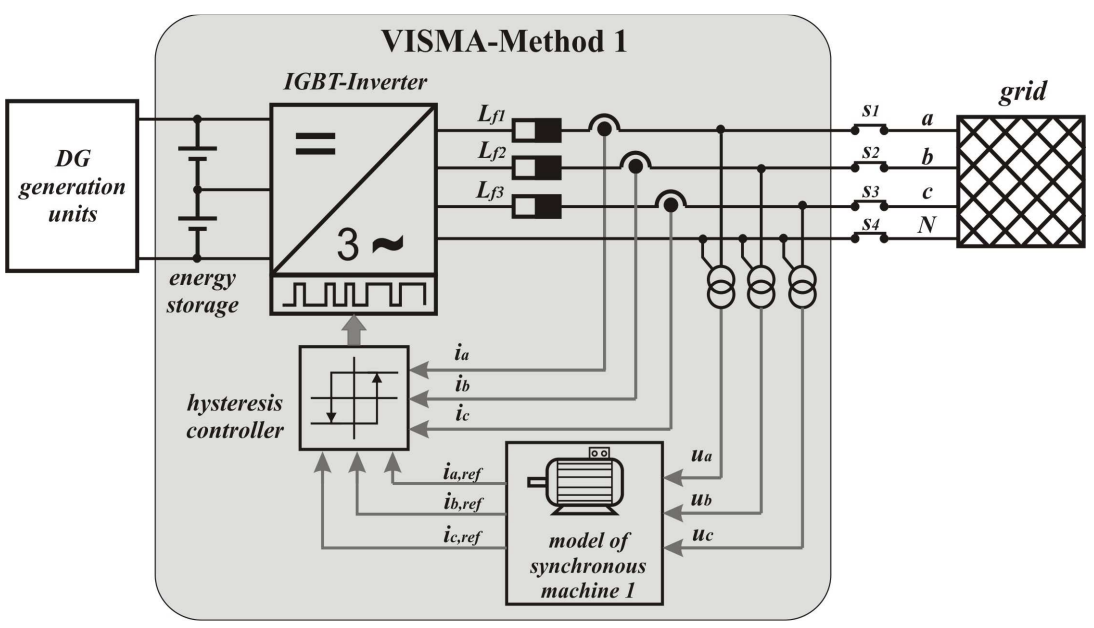
\includegraphics[width=8cm]{images/VISMA1Concept.png}
        \caption{}
        \label{fig:VISMA1Concept}
    \end{subfigure}

    \begin{subfigure}[b]{\textwidth}
        \centering
        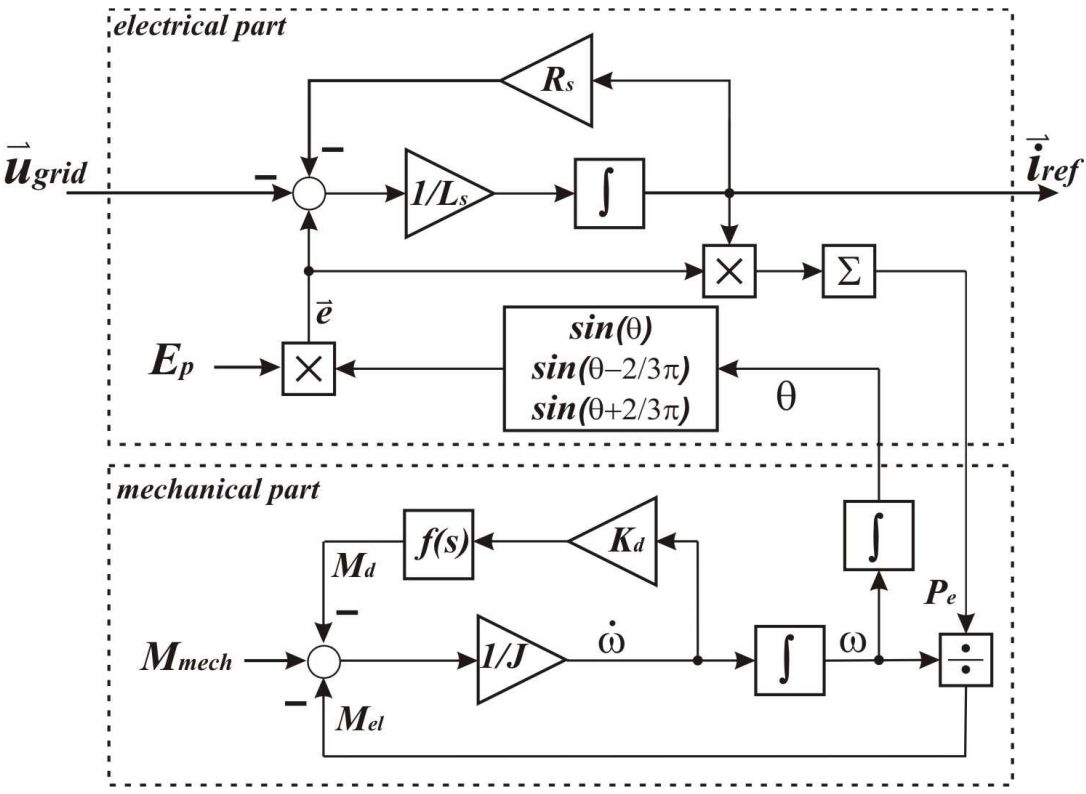
\includegraphics[width=5cm]{images/VISMA1block.png}
        \caption{}
        \label{fig:VISMA1block}
    \end{subfigure}
    \label{fig:VISMA1}
    \caption{VISMA-Method 1 (current-source-based control) \cite{chen2012comparison}. (a) Overall control scheme. (b) Model of synchronous machine 1.}
\end{figure}

\begin{figure}[ht!]
    \centering
    \begin{subfigure}[b]{\textwidth}
        \centering
        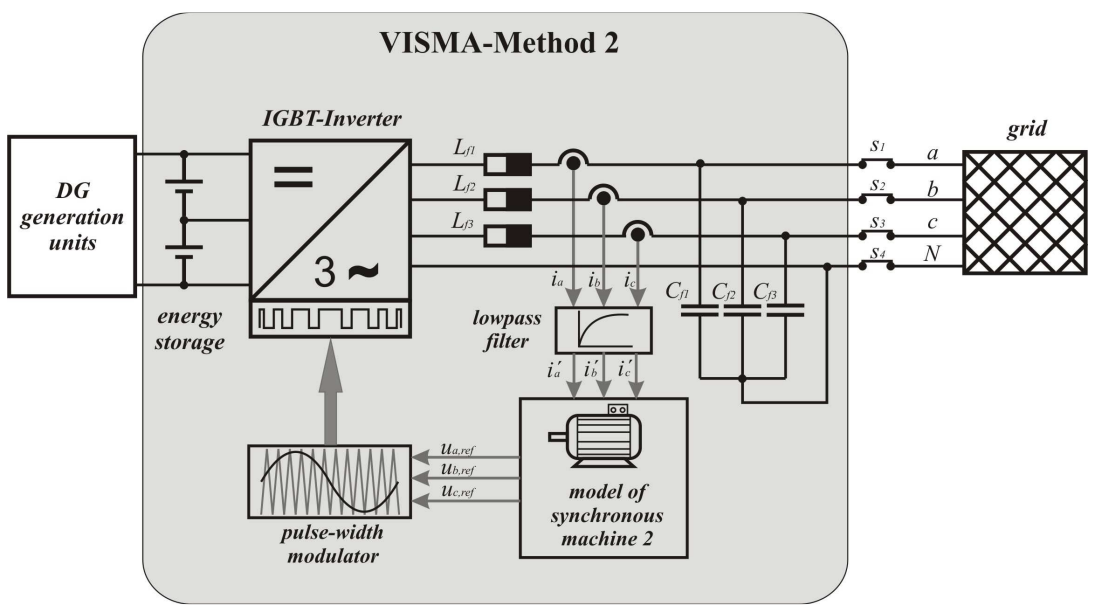
\includegraphics[width=8cm]{images/VISMA2Concept.png}
        \caption{}
        \label{fig:VISMA2Concept}
    \end{subfigure}

    \begin{subfigure}[b]{\textwidth}
        \centering
        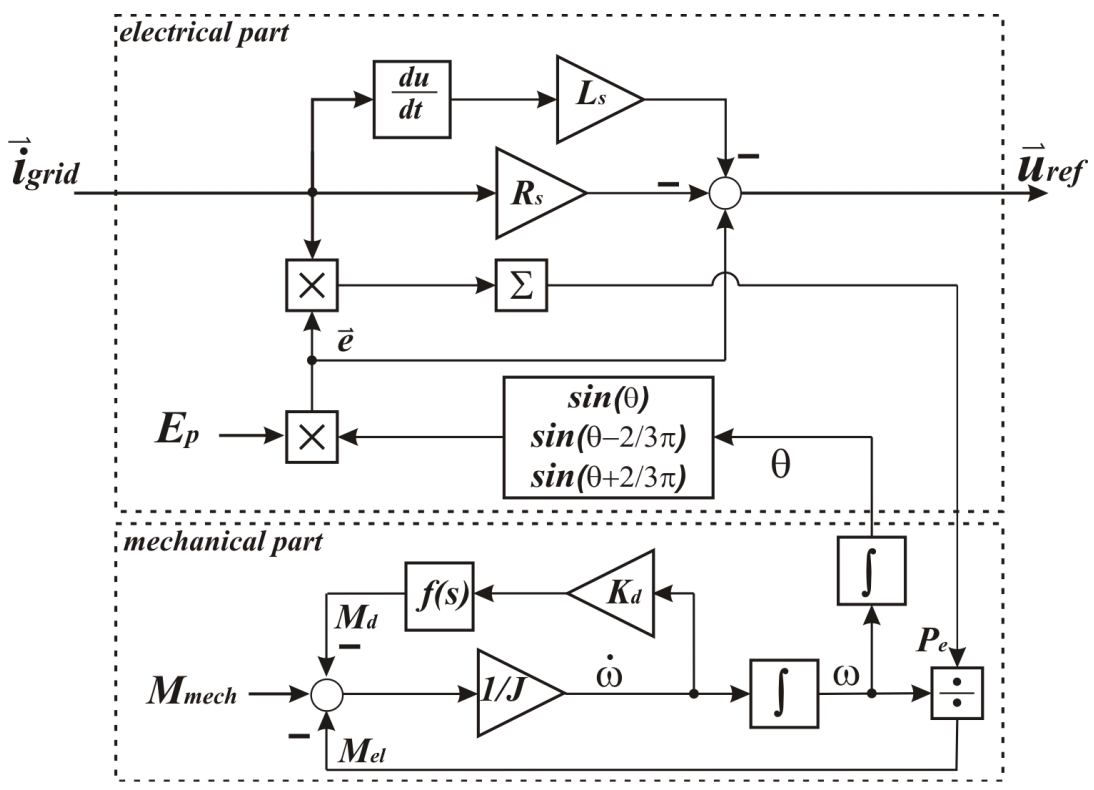
\includegraphics[width=5cm]{images/VISMA2block.png}
        \caption{}
        \label{fig:VISMA2block}
    \end{subfigure}
    \label{fig:VISMA2}
    \caption{VISMA-Method 2 (voltage-source-based control) \cite{chen2012comparison}.\\ (a) Overall control scheme. (b) Model of synchronous machine 2.}
\end{figure}

\newpage
The VISMA-Method 1 consists in measuring the grid voltage to feed the virtual
synchronous machine algorithm, which outputs a reference current analogous to
the stator current of a SG. The virtual synchronous machine algorithm consists
of an electrical part and a mechanical part that interact with each other. The
mechanical part corresponds to the rotor dynamics of the virtual synchronous
machine, and can be represented by the following equations:

\begin{equation*}
    \begin{aligned}
        M_{mech} - M_{el} &= \frac{1}{J} \frac{d\omega}{dt} + k_d f(s) \frac{d\omega}{dt}\\
        M_{el} &= \frac{P_{el}}{\omega}\\
        \theta &= \int \omega dt
    \end{aligned}
\end{equation*}
\noindent where $J$ is the moment of inertia, $k_d$ is the mechanical damping
factor, $f(s)$ is the phase compensation term, $\omega$ is the angular speed,
$\theta$ is the angular position and $M_{el}$ and $M_{mech}$ are the electrical
and mechanical torque.

$M_{mech}$ represents the action of the virtual governor, which is simplified as
being a control input to the system. The excitation system is also simplified,
being represented by an adjustable amplitude $E_p$, resulting in the following
induced electromotive force in the virtual stator.

\begin{equation*}
    \overrightarrow{e} =
    E_p\begin{bmatrix}e_a \\e_b \\ e_c\end{bmatrix} =
    E_p\begin{bmatrix}\sin{(\theta)} \\\sin{(\theta - \frac{2\pi}{3})} \\ \sin{(\theta + \frac{2\pi}{3})} \end{bmatrix}
\end{equation*}

Then, this induced electromotive force is used with the measured grid voltage in
the electrical part of the virtual synchronous machine model to calculate the
reference current, which is then used to drive the hysteresis controlled
converter. The electrical part of the synchronous machine model is represented
by the following equations.

\begin{equation*}
    \begin{aligned}
        e_a - u_a &= i_a^{ref}R_s + L_s\frac{di_a^{ref}}{dt}\\
        e_b - u_b &= i_b^{ref}R_s + L_s\frac{di_b^{ref}}{dt}\\
        e_c - u_c &= i_c^{ref}R_s + L_s\frac{di_c^{ref}}{dt}
    \end{aligned}
\end{equation*}
\noindent where $(u_a, u_b, u_c)$ are the measured grid voltage in each line,
$R_s$ and $L_s$ are the virtual stator resistance and inductance, respectively.

The working principle of the VISMA-Method 2 is exactly the same as of the
VISMA-Method 1, with the exception that the grid current is used instead of the
grid voltage for calculating the reference signal to drive the PWM based
converter. In other words, the electrical part of the synchronous machine model
is now represented by:

\begin{equation*}
    \begin{aligned}
        e_a - u_a^{ref} &= i_a R_s + L_s\frac{di_a}{dt}\\
        e_b - u_b^{ref} &= i_b R_s + L_s\frac{di_b}{dt}\\
        e_c - u_c^{ref} &= i_c R_s + L_s\frac{di_c}{dt}
    \end{aligned}
\end{equation*}
\noindent where $(i_a, i_b, i_c)$ are the measured grid current in each line.

It is important to highlight that the VISMA topology does not require a PLL and
uses a 5th order model of a SG, comprising of two mechanical state variables
($\theta$ and $\omega$) and 3 electromagnetic state variables (the stator
quantities). However, the damper and excitation windings are not taken into
consideration, and the transient and sub-transient dynamics are ignored.
This model does not consider possible saliency effects of the rotor.

Finally, it is important to highlight that the voltage-source-based VISMA
control can be considered as an upgraded grid-forming control, and the
current-source-based VISMA control can be considered as an upgraded grid-feeding
control.

\section{KHIs' VSM Topology}\label{sec:KHI}
KHI has proposed a current-source-based VSM topology in the $dq$-coordinate
frame\cite{hirase2013grid}, which control diagram is illustrated in the
following image.

\begin{figure}[ht!]
    \centering
    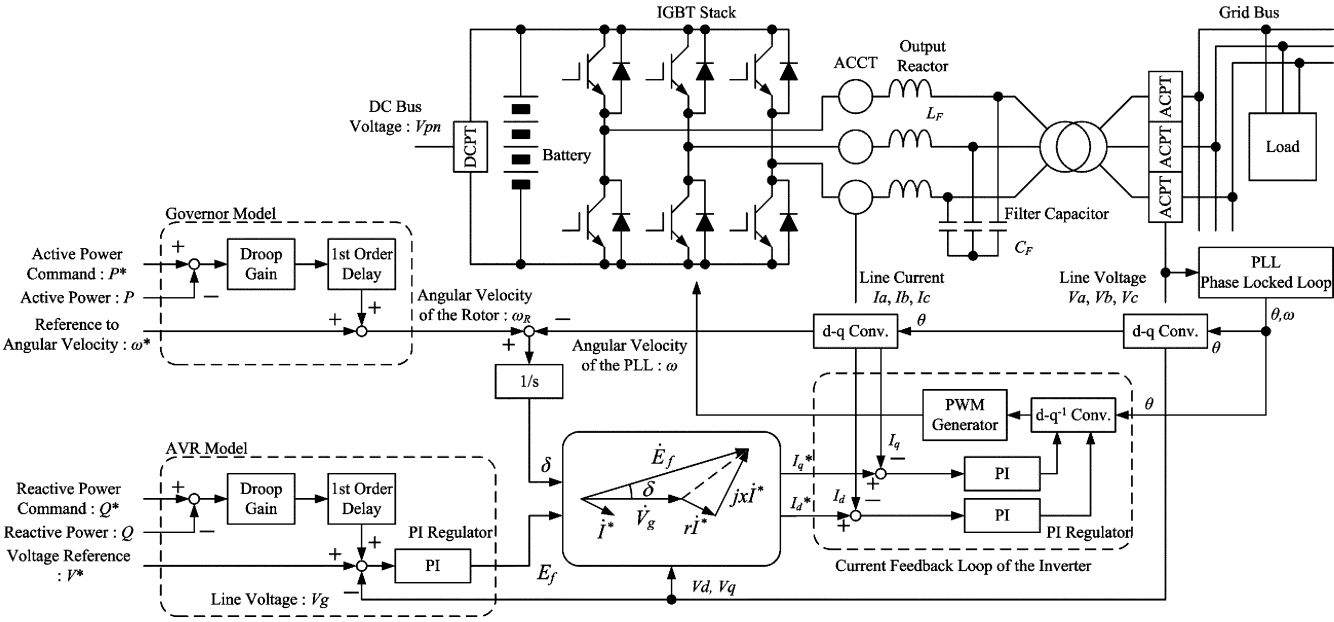
\includegraphics[width=14cm]{images/KHI.png}
    \caption{Control diagram of the VSM control developed by KHI\cite{hirase2013grid}.}
    \label{fig:KHI}
\end{figure}

In this model, the authors use phasor diagrams to express the relationship
between the phase voltage and line currents of the virtual generator, thus
ignoring the electrical dynamics. Moreover, the virtual generator is assumed to
be cylindrical, with the same synchronous reactance on the direct and quadrature
axes.

The model is composed of four main components: a PLL, an AVR, a virtual
governor, a virtual generator model, and a current feedback loop. The PLL is
used to detect the angular speed and angle of the grid side voltage of the
inverter's output filter, which is used in the $dq-$transformations.

The output active and reactive powers are also measured, and they are in the
virtual governor and AVR models to generate, respectively, the angular speed of
the virtual rotor, and the internal electromotive force. The virtual governor
and AVR models are simple PI controllers for active and reative power
regulation.

The outputs from the virtual governor and AVR are then used to compute the
reference current, which then passes through a current feedback loop to generate
the reference signal for the PWM modulation. Therefore, the VSM control by KHI
is a current-source-based grid-supporting control.

\section{ISE Lab's VSM Topology}
The Laboratory for Power Electronics and Electrical Drives (formely ISE Lab) at
Osaka University, which consists in emulating the SG swing equation
\cite{sakimoto2011stabilization,shintai2012reactive}. The following image
describes the block diagram of the Ise Lab's VSM topology.

\begin{figure}[ht!]
    \centering
    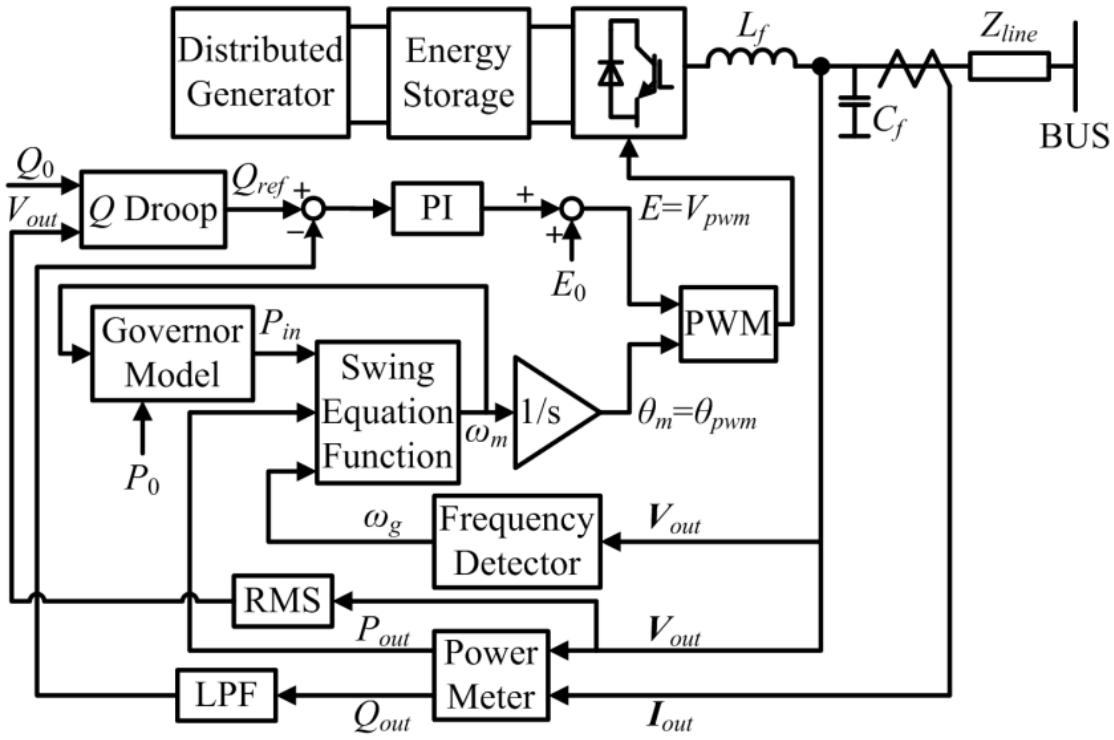
\includegraphics[width=14cm]{images/ISE.png}
    \caption{Control diagram of the VSM control developed by ISE Lab\cite{liu2016studies}.}
    \label{fig:ISE}
\end{figure}

This model consists in measuring the output current and voltage, which are then
used to compute the output active and reactive powers. The Frequency Detector
block corresponds to a PLL that is used to measure the bus frequency $\omega_g$
which is used to compute the virtual rotor frequency through the swing equation:

\begin{equation*}
    P_{in} - P_{out} = J\omega_m \frac{d\omega_m}{dt} + D(\omega_m - \omega_g)
\end{equation*}

The rotor frequency is used as a reference for the governor model and the PWM
inverter. Both the governor model and the Q Droop block are droop controllers
creating linear droops between active power and frequency, and between reactive
power and voltage, respectively.

It is important to highlight that no inner current or voltage loop is adopted in
this control scheme, so that the filter reactance is analogous to the stator
reactance of the VSM. This VSM control can be classified as a
voltage-source-based grid-supporting control.

\section{Synchronverter}\label{sec:synchronverter}

Another well-known VSM topology is the Synchronverter, which was proposed in
2009 by Qing-Chang Zhong and George Weiss. Initially, this topology was proposed
for a three-phase inverter operated using PWM and LC filters to reduce the
switching ripples \cite{zhong2011synchronverter}. The following figure
illustrates the overwall topology and control scheme of the Synchronverter.

\begin{figure}[ht!]
    \centering
    \begin{subfigure}[b]{\textwidth}
        \centering
        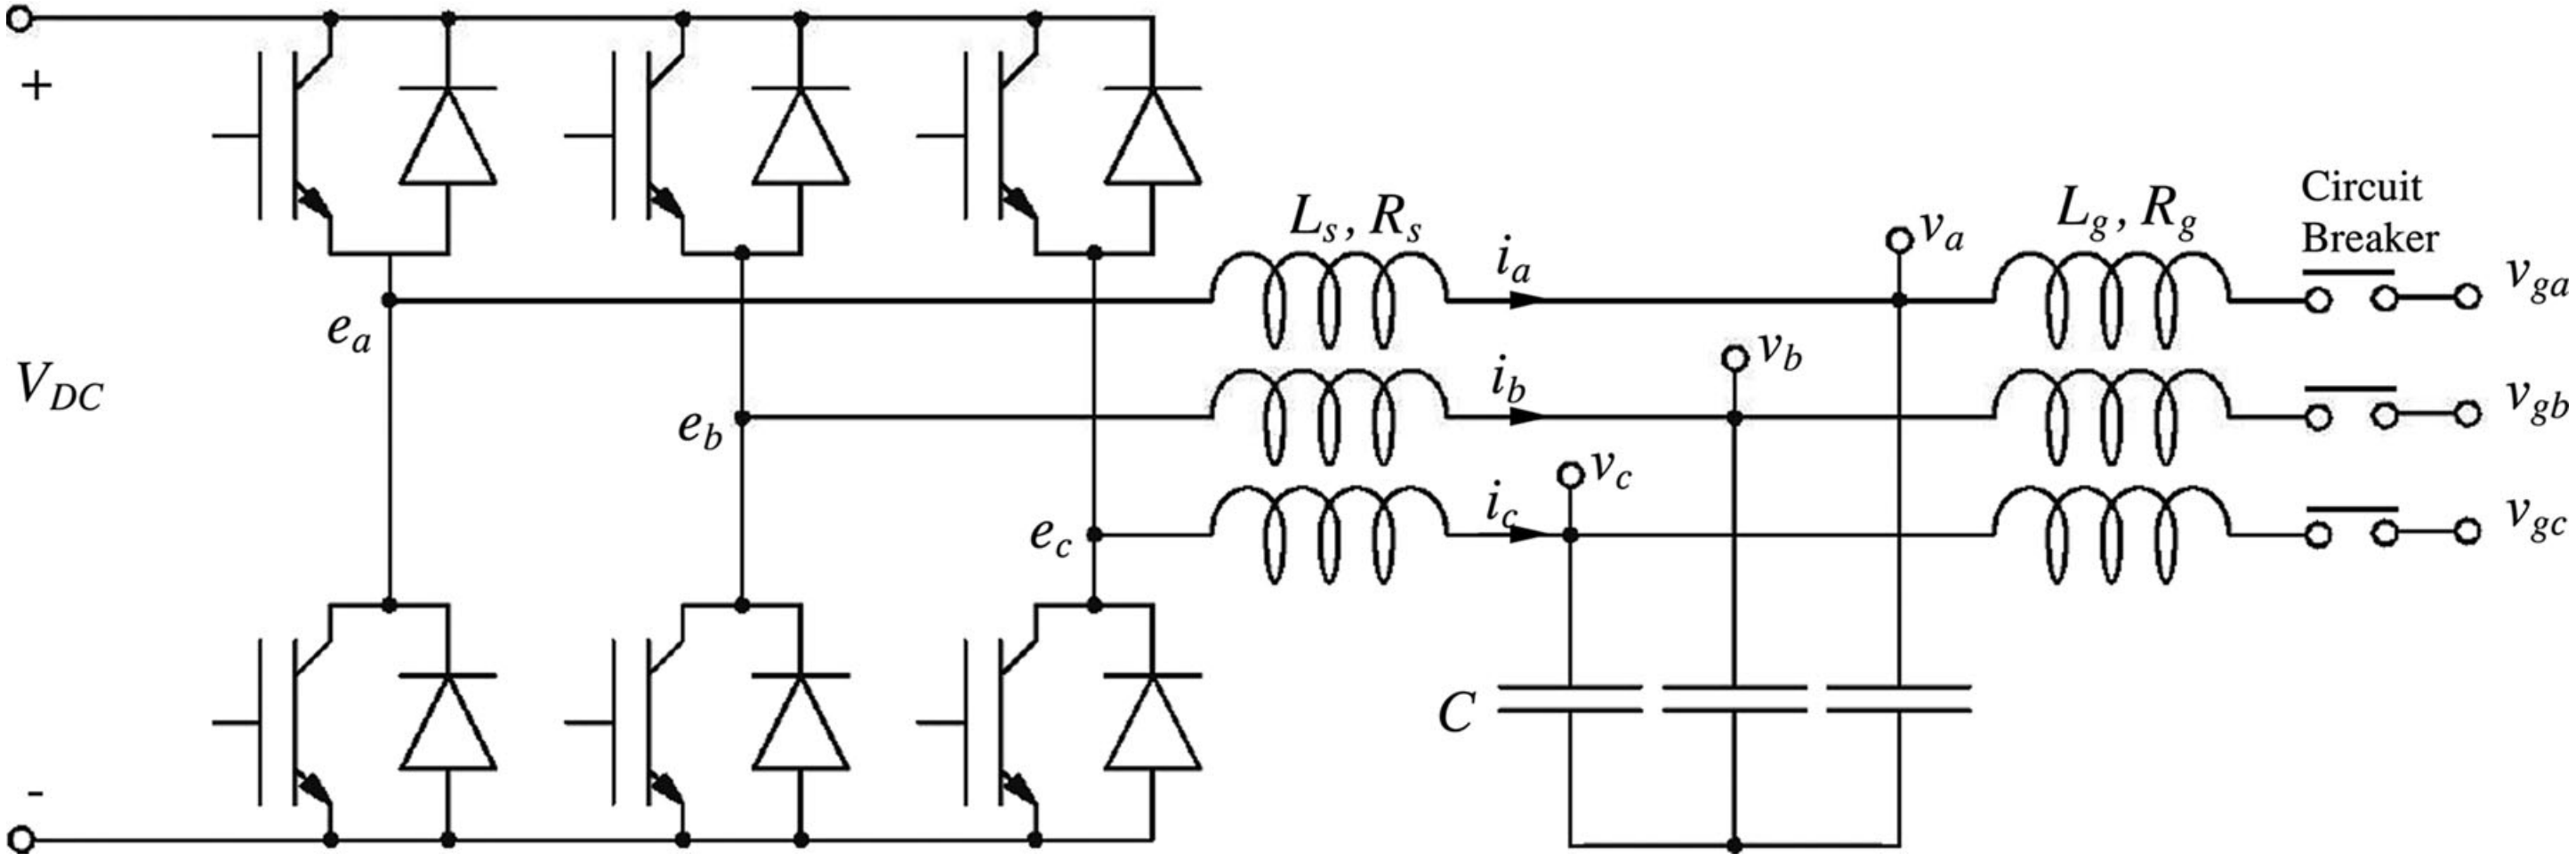
\includegraphics[width=12cm]{images/synchronverter_topology.png}
        \caption{}
        \label{fig:synchronverter_topology}
    \end{subfigure}

    \begin{subfigure}[b]{\textwidth}
        \centering
        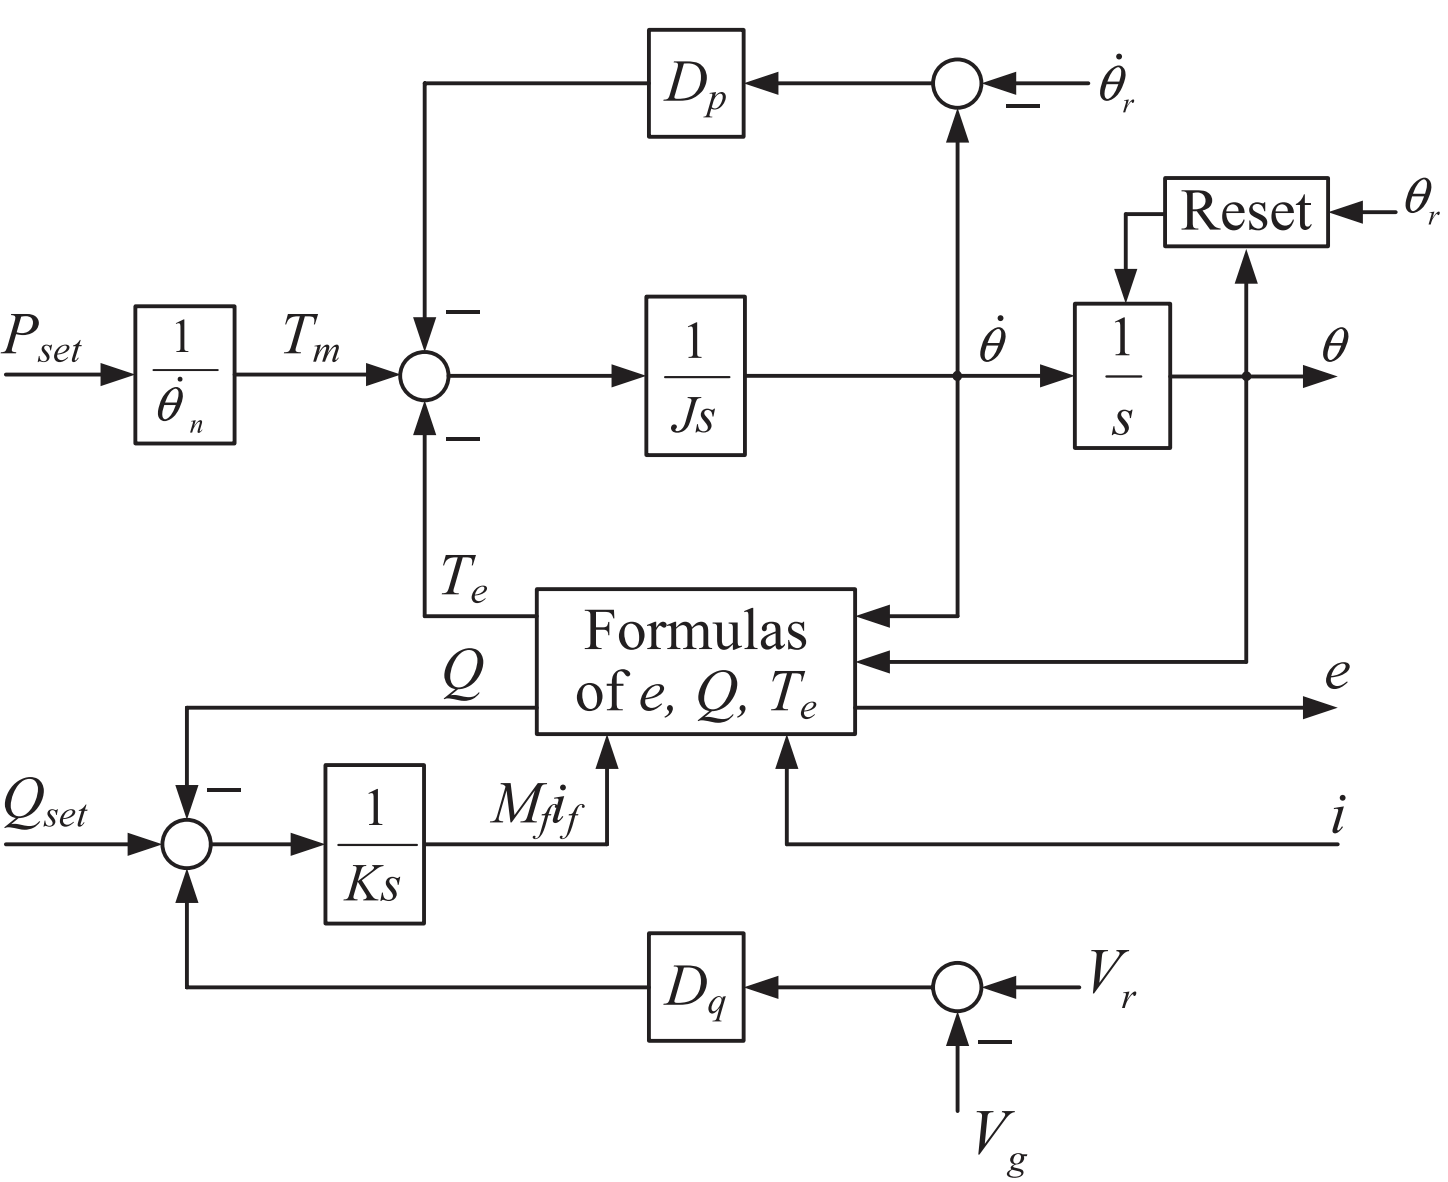
\includegraphics[width=8cm]{images/synchronverter_control.png}
        \caption{}
        \label{fig:synchronverter_control}
    \end{subfigure}
    \label{fig:synchronverter}
    \caption{Synchronverter (a) topology and (b) control scheme \cite{zhong2014self}}
\end{figure}

The modeling of the Synchronverter is based on the simplification of the SG
model by neglecting the damper windings in the rotor, and considering a round
rotor. Therefore, only an exciter winding in the rotor, and the three windings
in the stator are taken into consideration.

The system is designed based on the similarities between the dynamics of the
output filter of the converter and the stator windings of a SG. In other words,
the inverter's output filter dynamics match the dynamics of the stator windings
of a SG. Therefore, $L_s$ and $R_s$ in Figure \ref{fig:synchronverter_topology}
are equivalent to the reactance and impedance of the virtual generator, and the
capacitor voltage $(v_a, v_b, v_c)$ is equivalent to the stator terminal
voltage. The relationship between terminal current $i = (i_a, i_b, i_c)$ and
voltage $v = (v_a, v_b, v_c)$ is given by the follwing equation.

\begin{equation*}
    v = -R_s i - L_s \frac{di}{dt} + e
\end{equation*}

Therefore, the converter output voltage $e = (e_a, e_b, e_c)$ is controlled such
that it follows the same dynamics of a SG's back electromotive force (EMF):

\begin{equation*}
    e = M_f i_f \dot{\theta} \begin{bmatrix} \sin{(\theta)} \\ \sin{(\theta - \frac{2}{3}\pi)} \\ \sin{(\theta + \frac{2}{3}\pi)}\end{bmatrix} - M_f \frac{di_f}{dt} \begin{bmatrix} \cos{(\theta)} \\ \cos{(\theta - \frac{2}{3}\pi)} \\ \cos{(\theta + \frac{2}{3}\pi)}\end{bmatrix}
\end{equation*}

\noindent where $M_f$ is the mutual inductance between the virtual stator and
rotor, $i_f$ is the field excitation current, and $\theta$ is the virtual rotor
angle. Here, $i_f$ is used as an adjustable constant input, making the
derivative term to become zero:

\begin{equation*}
    e = M_f i_f \dot{\theta} \begin{bmatrix} \sin{(\theta)} \\ \sin{(\theta - \frac{2}{3}\pi)} \\ \sin{(\theta + \frac{2}{3}\pi)}\end{bmatrix}
\end{equation*}

On the other hand, $\theta$ and $M_f i_f$ are calculated according to active and
reactive power droop laws, respectively, as it can be seen in Figure
\ref{fig:synchronverter_control}. The active $P$ and reactive $Q$ powers are
calculated in the switching stage, corresponding to the multiplication between
$e$ and $i$.

Since the back EMF is used as a reference voltage for PWM modulation, the
synchronverter is a voltage-source-based grid-supporting control method, and due
to the lack of current control gives rise to a potential issue related to
excessive high inrush fault current\cite{shuai2017characteristics}.

\section{Cascaded Virtual Synchronous Machine}\label{sec:CSVSM}

In 2013, a new VSM implementation approach was proposed by Salvatore D'Arco, Jon
Are Suul and Olav B. Fosso\cite{darco2013control,darco2014small,darco2015vsm}.
In this thesis we call this implementation as Cascaded Virtual Synchronous
Machine (CVSM), due to the fact that it includes two cascaded PI controls for
voltage and current regulation. It is a voltage-source-based grid-supporting
control method, and an overview of the system configuration and control scheme
is illustrated in the Figure \ref{fig:CVSM}.

\begin{figure}[ht!]
    \centering
    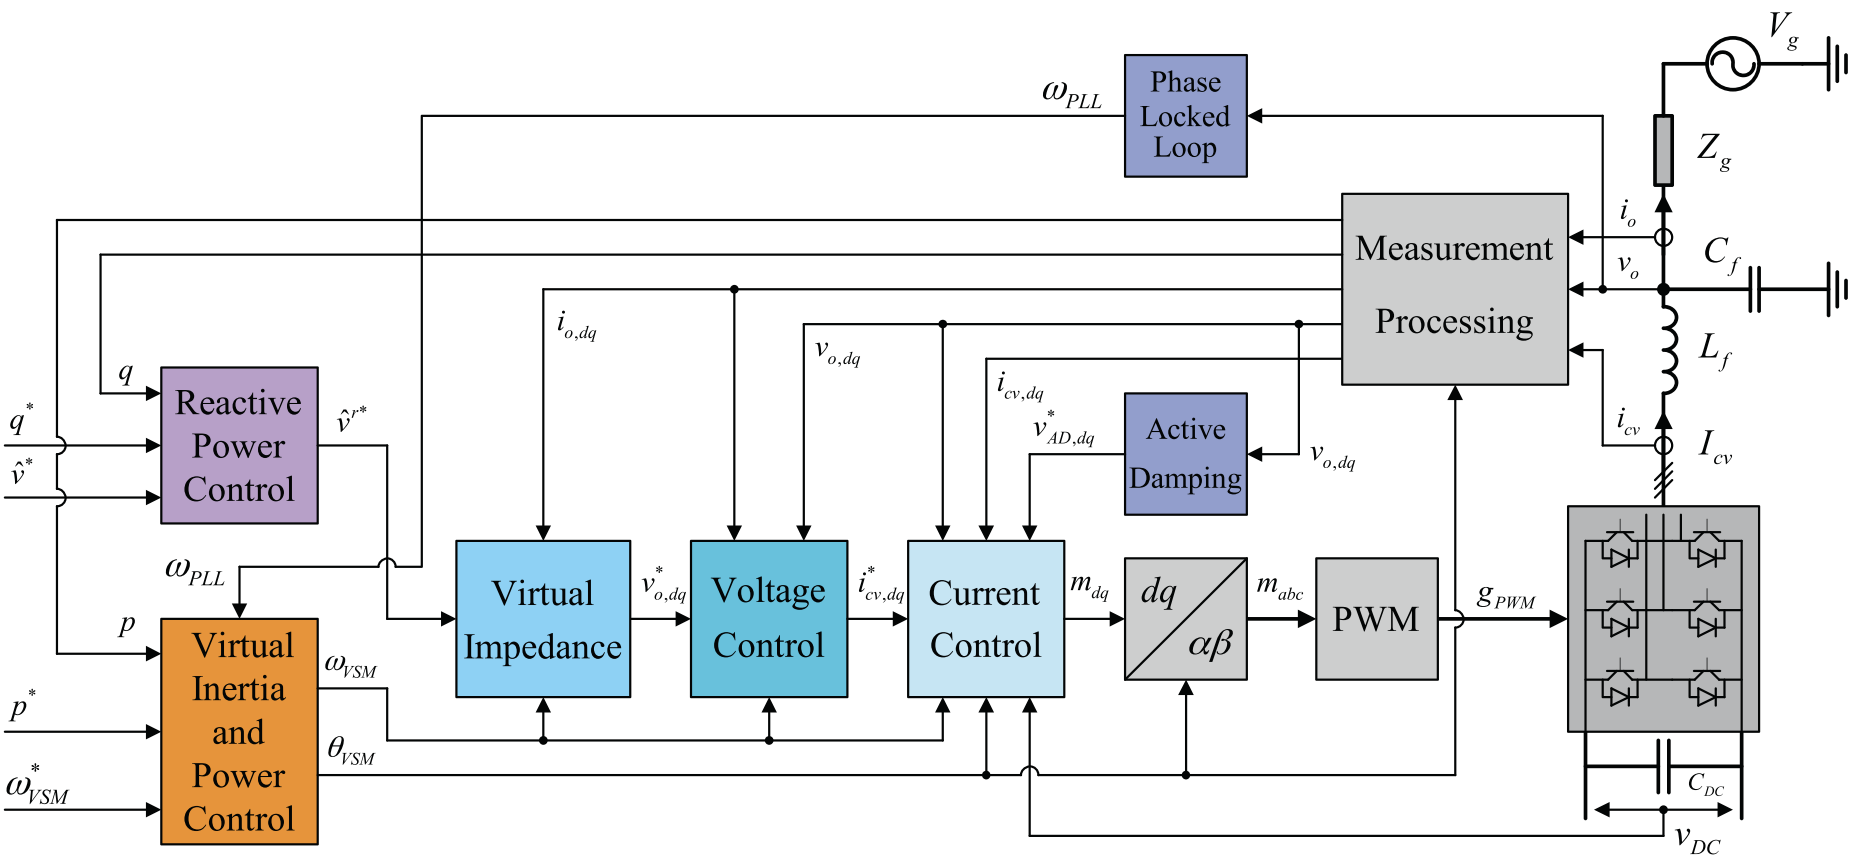
\includegraphics[width=12cm]{images/CVSM.png}
    \caption{CVSM system topology and control scheme\cite{darco2015vsm}.}
    \label{fig:CVSM}
\end{figure}

The system is modeled in the $dq-$frame, and the synchronization is realized by
the power balance of the VSM swing equation. In other words, the coordinate
transformations use the internal angle $\omega_{VSM}$ corresponding to the angle
position of the virtual rotor. The presence of a PLL therefore does not
introduce any instability problem.

The Virtual Inertia and Power Control block corresponds to the swing equation
emulation, with the damping power/torque being proportional to the difference
between  the virtual rotor frequency and the grid frequency, thus the need of a
PLL for estimation of the grid frequency. It is important to highlight that the 
damping power/torque is defined slightly differently from traditional SG
modeling theory \cite{sauer2017power, kundur2022power}. Figure
\ref{fig:CVSM_power} illustrates the control scheme of the Virtual Inertia and
Power Control block.

\begin{figure}[ht!]
    \centering
    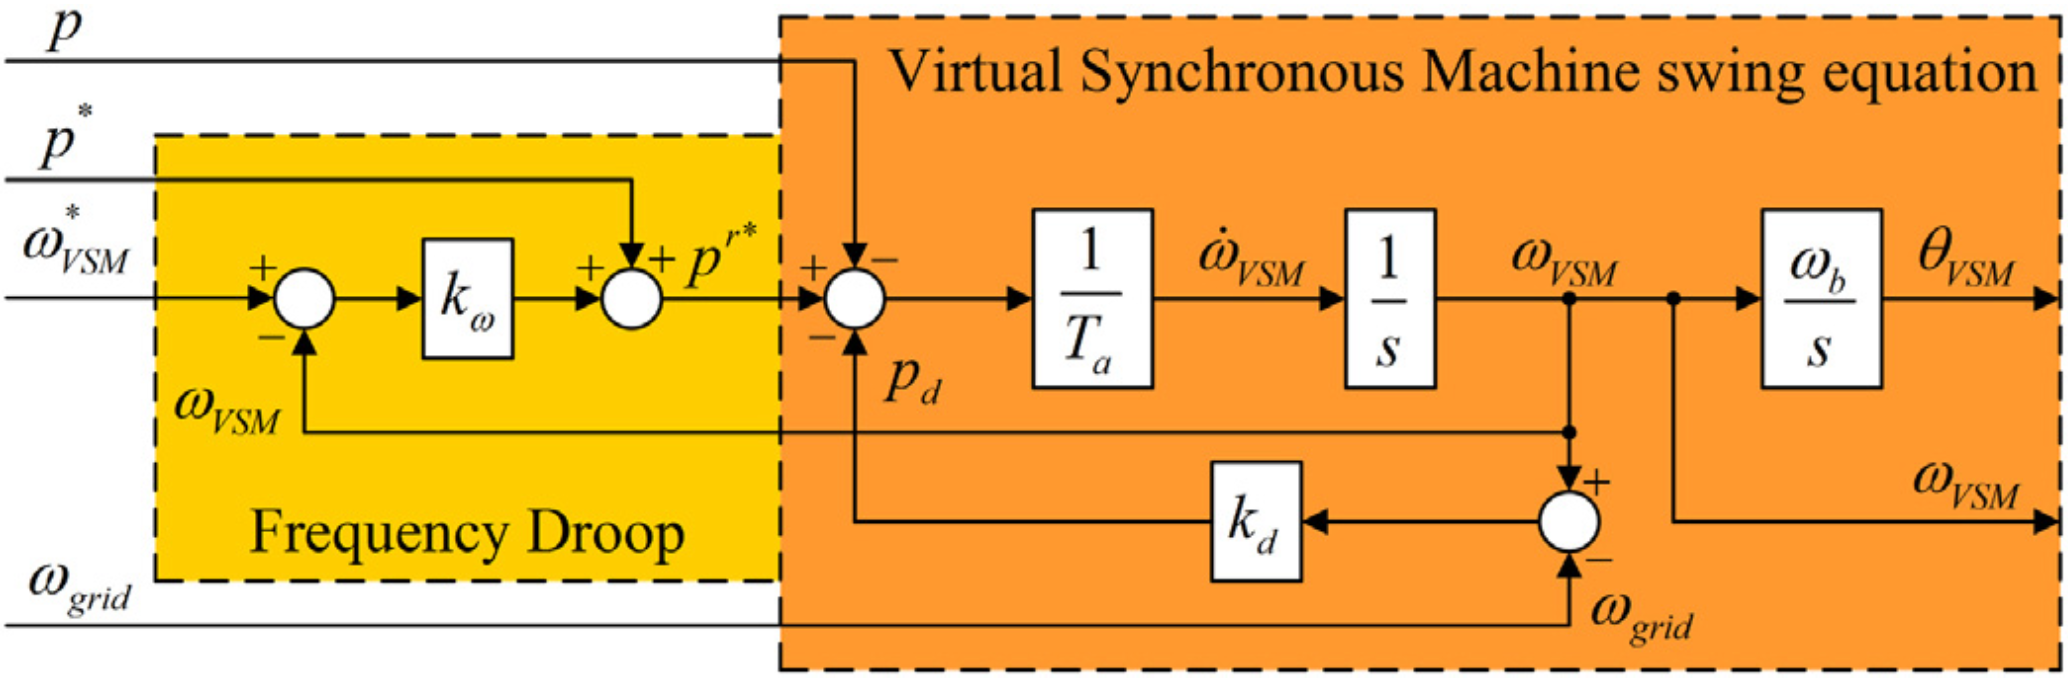
\includegraphics[width=12cm]{images/CVSM_power.png}
    \caption{Control scheme of the Virtual Inertia and Power Control block\cite{darco2015vsm}.}
    \label{fig:CVSM_power}
\end{figure}

On the other hand, the reactive power control is implemented in a similar manner
as the other VSM implementations, consisting in a droop law for the reactive
power. The resulting signal is the voltage amplitude reference $\hat{v}^r*$,
which is passed through a virtual impedance before it is used as a reference for
the PWM modulation. This virtual impedance is analogous to the SG stator
impedance and it is used for reducing the sensitivity of the VSM to small
disturbances.

Finally, the resulting voltage reference vector $v_0*$ is passed through a
cascaded PI controller with feedforward terms to provide decoupling of the $dq$
terms and allow for current and voltage limitation. Moreover, an additional
voltage reference voltage magnitude corresponding to an active damping technique
is added to the output of of the PI current controller before being used for PWM
modulation. The active damping is used for supressing oscillations in the LC
filter. The overall cascaded PI controller is illustrated in the Figure
\ref{fig:CVSM_cascaded}.

\begin{figure}[ht!]
    \centering
    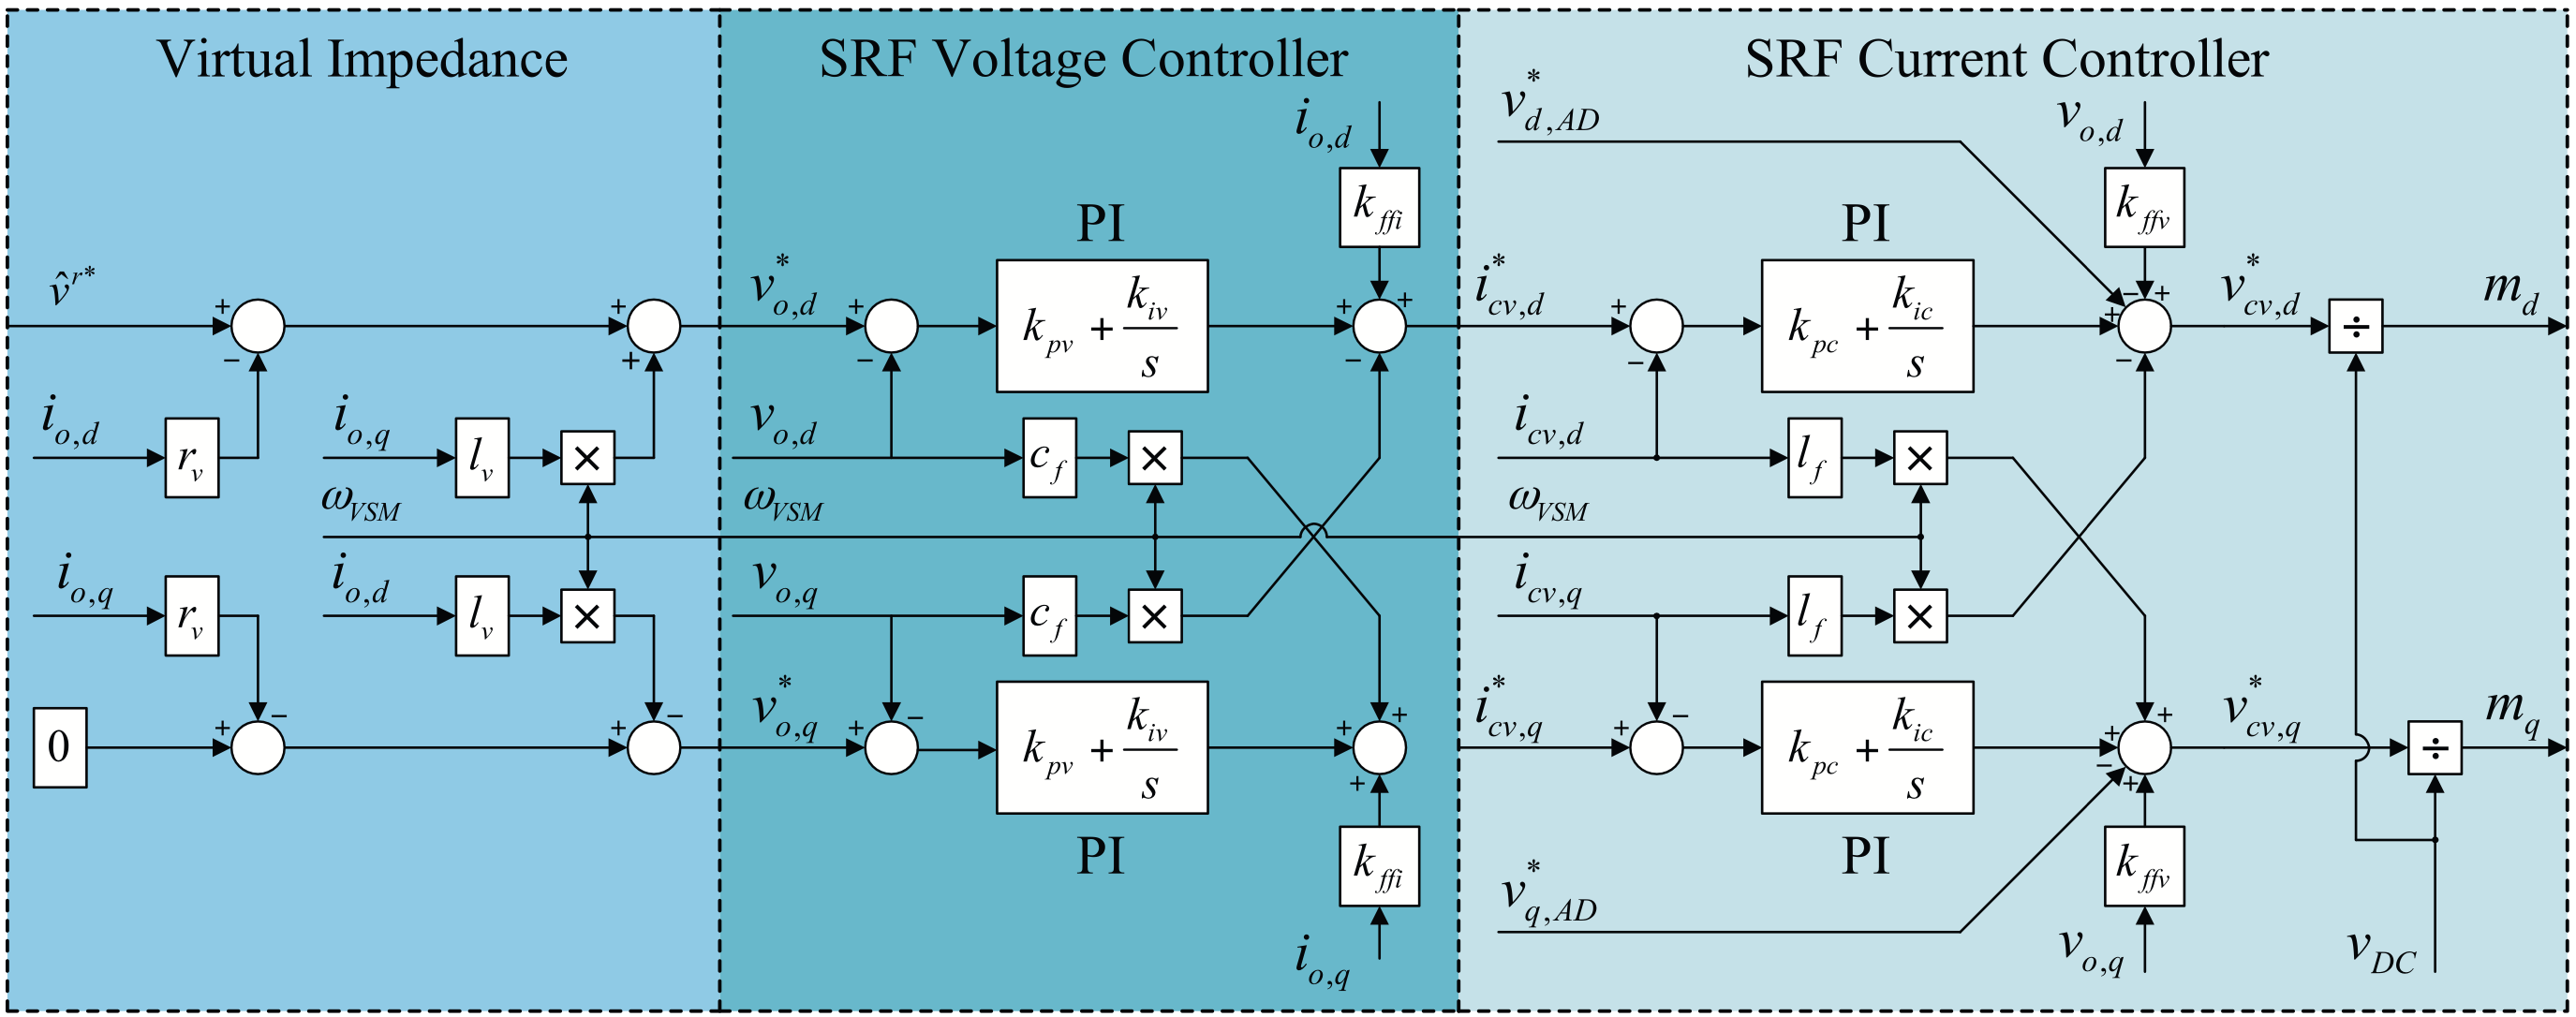
\includegraphics[width=12cm]{images/CVSM_cascaded.png}
    \caption{Virtual impedance and cascaded PI voltage control block scheme\cite{darco2015vsm}.}
    \label{fig:CVSM_cascaded}
\end{figure}

\newpage
\section{Summary of VSM Topologies}

The following table summarizes the VSM topologies discussed in this Chapter
according to characteristics that can be compared with SGs, such as control
method, consideration of virtual damper windings, virtual impedance, need for
PLL and overcurrent protection. 

\begin{table}[ht!]
    \centering
    \resizebox{\textwidth}{!}{
        \begin{tabular}{llllll}
        \toprule
        \textbf{Topology} & \textbf{Control method} & \textbf{Virtual damper windings} & \textbf{Has virtual impedance?} & \textbf{Need PLL?} & \textbf{Has overcurrent protection?} \\ 
        \midrule
        VSYNC            & current-source-based & 0 & No & Yes & Yes  \\
        VISMA-Method 1   & current-source-based & 0 & Yes & No & No  \\
        VISMA-Method 2   & voltage-source-based & 0 & Yes & No & No \\
        KHI              & current-source-based & 0 & Yes & Yes & Yes  \\
        ISE              & voltage-source-based & 0 & No & Yes & No \\
        Synchronverter   & voltage-source-based & 0 & No & No & Yes \\
        CVSM             & voltage-source-based & 0 & Yes & Yes & Yes  \\
        \bottomrule
        \end{tabular}
    }
    \caption{\centering Summary of VSM topologies.}
    \label{tab:topologies_summary}
\end{table}

As established in Section \ref{sec:control_methods}, current-source-based
grid-supporting control methods lack the capability to provide voltage support
in weak grids with a high presence of Inverter-Based Resources (IBRs).
Consequently, this thesis will not consider current-source-based grid-support
control topologies.

Virtual impedance emulates the synchronous impedance behavior of traditional SGs
and is instrumental in shaping system dynamics. Employing a PLL can adversely
affect control performance in weak AC systems; therefore, PLL-free topologies
are preferable. Furthermore, considering the susceptibility of power converters
to high current levels, overcurrent protection is a critical safety feature.

According to Table \ref{tab:topologies_summary}, the CVSM topology meets all the
stated requirements. Although it typically requires a PLL, it is implemented not
for synchronization, and some authors have implemented this topology without the
use of PLL \cite{tayyebi2020power}. Notably, this topology does not inherently
include virtual damper windings.

Damper windings in SGs are essential for damping oscillations and suppressing
hunting, enhancing system stability \cite{sauer2017power,kundur2022power}. The
primary distinction between low-order SG models (like the classical and 1-axis
models) and high-order models (such as the 2-axis and Park's models) lies in the
inclusion of damper windings. This feature has been incorporated into the CVSM
topology in recent studies \cite{zhang2013vsm,ma2017vsg}.

This thesis will adopt the CVSM topology with the integration of virtual damper
windings, following the approach used by \cite{zhang2013vsm, ma2017vsg}. This
will facilitate a comprehensive comparison of the dynamic characteristics
between SGs and VSMs of varying orders and assess the significance of including
virtual damper windings.